
\documentclass[main.tex,fontsize=8pt,paper=a4,paper=portrait,DIV=calc,]{scrartcl}
% Document
\usepackage[T1]{fontenc}
\usepackage[utf8]{inputenc}
\usepackage[dvipsnames]{xcolor}
\usepackage[nswissgerman,english]{babel} 
\usepackage{hyperref}
\renewcommand{\familydefault}{\sfdefault}

% Format
\usepackage[top=5mm,bottom=1mm,left=5mm,right=5mm]{geometry}
%\setlength{\headheight}{\baselineskip}
%\setlength{\headsep}{0mm}

%\usepackage{scrlayer-scrpage}
%\clearpairofpagestyles
%\chead{{\bfseries\TITLE, \AUTHOR, \pagename~\thepage}}

%\addtokomafont{pagehead}{\upshape}

\usepackage{multicol}
\setlength{\columnsep}{2mm}
\setlength{\columnseprule}{0.1pt}

% Math
\usepackage{amsmath}
\usepackage{amssymb}
\usepackage{amsfonts}

% Code
\usepackage{fancyvrb, etoolbox, listings, xcolor}
%\usemintedstyle{bw}

%\newminted[shell]{bash}{
%fontsize=\footnotesize,
%fontfamily=tt,
%breaklines=true,
%frame=single,
%framerule=0.1pt,
%framesep=2mm,
%tabsize=2
%}
%\newminted{css}{
%breaklines=true,
%tabsize=4,
%autogobble=true,
%escapeinside=||,
%stripall=true,
%stripnl=true,
%}

    \definecolor{lightgray}{rgb}{0.95, 0.95, 0.95}
    \definecolor{darkgray}{rgb}{0.4, 0.4, 0.4}
    \definecolor{purple}{rgb}{0.65, 0.12, 0.82}
    \definecolor{ocherCode}{rgb}{1, 0.5, 0} % #FF7F00 -> rgb(239, 169, 0)
    \definecolor{blueCode}{rgb}{0, 0, 0.93} % #0000EE -> rgb(0, 0, 238)
    \definecolor{greenCode}{rgb}{0, 0.6, 0} % #009900 -> rgb(0, 153, 0)
    \definecolor{teal}{rgb}{0.0, 0.5, 0.5}

\lstdefinestyle{code}{
    identifierstyle=\color{black},
    keywordstyle=\color{blue}\bfseries\small,
    ndkeywordstyle=\color{greenCode}\bfseries\small,
    stringstyle=\color{ocherCode}\ttfamily\small,
    commentstyle=\color{teal}\ttfamily\textit\small,
    basicstyle=\ttfamily\small,
    breakatwhitespace=false,         
    breaklines=true,                 
    captionpos=b,                    
    keepspaces=true,                 
    showspaces=false,                
    showstringspaces=false,
    showtabs=false,                  
    tabsize=2,
    belowskip=-5pt
}



% Images
\usepackage{graphicx}
\newcommand{\pic}{\includegraphics[scale=0.3]}
\graphicspath{{Screenshots/}{../Screenshots}}
\makeatletter
\def\pictext#1#2{%
    \@ifnextchar[{%
    \pictext@iiiii{#1}{#2}%
    }{%
      \pictext@iiiii{#1}{#2}[0.5,0.4,0.3]% Default is 5
    }%
}
\def\pictext@iiiii#1#2[#3,#4,#5]{\begin{minipage}{#3\textwidth}\includegraphics[scale=#4]{#1}\end{minipage}\begin{minipage}{#5\textwidth}#2\end{minipage}}
\def\minipg#1#2{%
    \@ifnextchar[{%
    \minipg@iiii{#1}{#2}%
    }{%
      \minipg@iiii{#1}{#2}[0.3,0.6]% Default is 5
    }%
}
\def\minipg@iiii#1#2[#3,#4]{\vspace{0.8mm}\begin{minipage}{#3\textwidth}#1\end{minipage}\begin{minipage}{#4\textwidth}#2\end{minipage}{\vspace{0.8mm}}}
\makeatother

%\newenvironment{minty}[2]% environment name
%{% begin code
%  \begin{minipage}{#1}
%  \begin{minted}{#2}
%}%
%{% end code
%  \end{minted}
%  \end{minipage}
%  \end{minty}\ignorespacesafterend
%} 

% Smaller Lists
\usepackage{enumitem}
\setlist[itemize,enumerate]{leftmargin=3mm, labelindent=0mm, labelwidth=1mm, labelsep=1mm, nosep}
\setlist[description]{leftmargin=0mm, nosep}
\setlength{\parindent}{0cm}

% Smaller Titles
\usepackage[explicit]{titlesec}

%% Color Boxes
\newcommand{\sectioncolor}[1]{\colorbox{black!60}{\parbox{0.989\linewidth}{\color{white}#1}}}
\newcommand{\subsectioncolor}[1]{\colorbox{black!50}{\parbox{0.989\linewidth}{\color{white}#1}}}
\newcommand{\subsubsectioncolor}[1]{\colorbox{black!40}{\parbox{0.989\linewidth}{\color{white}#1}}}
\newcommand{\paragraphcolor}[1]{\colorbox{black!30}{\parbox{0.989\linewidth}{\color{white}#1}}}
\newcommand{\subparagraphcolor}[1]{\colorbox{black!20}{\parbox{0.989\linewidth}{\color{white}#1}}}

%% Title Format
\titleformat{\section}{\vspace{0.5mm}\bfseries}{}{0mm}{\sectioncolor{\thesection~#1}}[{\vspace{0.5mm}}]
\titleformat{\subsection}{\vspace{0.5mm}\bfseries}{}{0mm}{\subsectioncolor{\thesubsection~#1}}[{\vspace{0.5mm}}]
\titleformat{\subsubsection}{\vspace{0.5mm}\bfseries}{}{0mm}{\subsubsectioncolor{\thesubsubsection~#1}}[{\vspace{0.5mm}}]
\titleformat{\paragraph}{\vspace{0.5mm}\bfseries}{}{0mm}{\paragraphcolor{\theparagraph~#1}}[{\vspace{0.5mm}}]
\titleformat{\subparagraph}{\vspace{0.5mm}\bfseries}{}{0mm}{\subparagraphcolor{\thesubparagraph~#1}}[{\vspace{0.5mm}}]

%% Title Spacing
\titlespacing{\section}{0mm}{0mm}{0mm}
\titlespacing{\subsection}{0mm}{0mm}{0mm}
\titlespacing{\subsubsection}{0mm}{0mm}{0mm}
\titlespacing{\paragraph}{0mm}{0mm}{0mm}
\titlespacing{\subparagraph}{0mm}{0mm}{0mm}

%% format cells
\usepackage[document]{ragged2e}
\usepackage{array, makecell}
\renewcommand{\arraystretch}{2}
\newcommand{\mc}{\makecell[{{m{1\linewidth}}}]}



\lstdefinelanguage{JavaScript}{
  keywords={break, case, catch, continue, debugger, default, delete, do, else, false, finally, for, function, if, in, instanceof, new, null, return, switch, this, throw, true, try, typeof, var, void, while, with},
  morecomment=[l]{//},
  morecomment=[s]{/*}{*/},
  morestring=[b]',
  morestring=[b]",
  ndkeywords={class, export, boolean, throw, implements, import, this},
  keywordstyle=\color{blue}\bfseries,
  ndkeywordstyle=\color{darkgray}\bfseries,
  identifierstyle=\color{black},
  commentstyle=\color{purple}\ttfamily,
  stringstyle=\color{red}\ttfamily,
  sensitive=true
}

\lstdefinelanguage{CSS}{
    sensitive=true,
    keywords={%
    % JavaScript
    typeof, new, true, false, catch, function, return, null, catch, switch, var, if, in, while, do, else, case, break,
    % HTML
    html, title, meta, style, head, body, script, canvas,
    % CSS
    color:, border-radius:, border:, transform:, -moz-transform:, transition-duration:, transition-property:,
    transition-timing-function, background:, background-size:, background-color:, background-image:, background-origin:, background-repeat:, background-position:, background-attachement:, border:, border-box:, border-width:, border-color:, border-bottom:, border-style:, border-radius:, border-spacing:, border-collapse:, text-transform:, text-decoration-thickness:, text-align:, text-indent:, text-shadow:, text-justify:, text-overflow:, text-decoration:, text-align-last:, text-decoration-line:, text-decoration-color:, text-decoration-style:, margin:, padding:, 
    },
    % http://texblog.org/tag/otherkeywords/
    otherkeywords={<, >},   
    ndkeywords={class, export, boolean, throw, implements, import, this},   
    comment=[s]{/*}{*/},
    morecomment=[l]//,
    morecomment=[s]{<!}{>},
    morestring=[b]',
    morestring=[b]",    
    alsoletter={-},
    alsodigit={:}
}

\lstdefinelanguage{HTML}{
    sensitive=true,
    keywords={%
    % JavaScript
    typeof, new, true, false, catch, function, return, null, catch, switch, var, if, in, while, do, else, case, break,
    % HTML
    html, title, meta, style, head, body, script, canvas,
    % CSS
    color:, border-radius:, border:, transform:, -moz-transform:, transition-duration:, transition-property:,
    transition-timing-function, background:, background-size:, background-color:, background-image:, background-origin:, background-repeat:, background-position:, background-attachement:, border:, border-box:, border-width:, border-color:, border-bottom:, border-style:, border-radius:, border-spacing:, border-collapse:, text-transform:, text-decoration-thickness:, text-align:, text-indent:, text-shadow:, text-justify:, text-overflow:, text-decoration:, text-align-last:, text-decoration-line:, text-decoration-color:, text-decoration-style:, margin:, padding:, 
    },
    % http://texblog.org/tag/otherkeywords/
    ndkeywords={class, export, boolean, throw, implements, import, this},   
    comment=[s]{/*}{*/},
    morecomment=[l]//,
    morecomment=[s]{<!--}{-->},
    morestring=[b]',
    morestring=[b]",    
    alsoletter={-},
    %otherkeywords={<, >},   
    alsodigit={:}
}

\newcommand{\TITLE}{Web Engineering 2}
\newcommand{\AUTHOR}{Fabio Lenherr}
\setcounter{tocdepth}{1}

\begin{document}
\tableofcontents

\lstset{
    language=JavaScript,
    style=code,
}

\section{NodeJS and other WebServers}
This is the interface between the operating system and the actual website itself. -> Apache\newline
\begin{itemize}
\item \textcolor{green}{Runs everywhere}
\item \textcolor{green}{async with events}
\item \textcolor{green}{easy to deploy}
\item \textcolor{green}{Lots of APIs for different usecases}\newline
  HTTP/HTTPS, URL, FileSystem, Console, UDP, Cryptography, DNS
\item \textcolor{green}{modular}
\item \textcolor{green}{not that much "magic"}\newline
  you need to write more yourself
\end{itemize} 
\textcolor{red}{negative: IT IS JS, FFS}\dots

\subsection{Async via events}
The idea of events is \emph{essentially a queue that doesn't block actual functionality}, this means that your UI still does what it should, as it will be prioritized compared to async functionaity.\newline
\textcolor{teal}{Just like bevy, the events are handled in the next frame, or more precise \emph{whenever there is nothing else to do}.}\newline
This means we will get the illusion of async/multi-threading, without js actually being able to do so.

\subsection{Callback hell with async events}
If you constantly need to check for finished events, then you will end up with unreadable code.\newline
\textcolor{green}{The solution is simple: Promises}\newline
The default in NodeJS is still callbacks, but there is work on this to change.\newline
Example for callback 
\begin{lstlisting}
button.addEventListener('click', function (event) {
  console.log("1. subscription");
});
\end{lstlisting}

\subsection{Example for NodeJS}
\begin{lstlisting}
const http = require('node:http'); // lua?

const hostname = '127.0.0.1';
const port = 3000;

const server = http.createServer((req, res) => {
  res.statusCode = 200; // HTTP response
  res.setHeader('Content-Type', 'text/plain');
  res.end('Hello, World!\n');
});

server.listen(port, hostname, () => {
  console.log(`Server running at http://${hostname}:${port}/`);
});
\end{lstlisting}

\section{Modules}
\subsection{NPM}
\begin{itemize}
\item \textcolor{purple}{npm init}\newline
  \begin{itemize}
  \item \textcolor{black}{-g for global installation}
  \item \textcolor{black}{--save-dev for a module that will only be used during development}
  \end{itemize} 
\item \textcolor{purple}{}
\item \textcolor{purple}{item 3}
\item \textcolor{purple}{item 4}
\end{itemize}

\subsection{Exporting Modules}
\begin{lstlisting}
function add() { return ++counter; }
function get() { return counter; }
// default export
export default {count: add, get: get};
// named
export {add, get};
\end{lstlisting}

\subsection{Importing Modules}
\begin{lstlisting}
// default
import counterA from './counter.mjs';
// Named
import {add, get} from './counter.mjs';
\end{lstlisting}

\subsection{package.json}
\begin{lstlisting}
{
  "name": "my_package",
  "description": "",
  "version": "1.0.0",
  "main": "index.js",
  "type": "module",
  "scripts": {
    "test": "echo \"Error: no test specified\" && exit 1"
  },
  "repository": {
    "type": "git",
    "url": "https://github.com/mgfeller/my_package.git"
  },
  "keywords": [],
  "author": "",
  "license": "ISC",
  "bugs": {
    "url": "https://github.com/mgfeller/my_package/issues"
  },
  "homepage": "https://github.com/mgfeller/my_package"
}
\end{lstlisting}

\subsection{package-lock.json}
\textcolor{teal}{This handles dependency problems, where one dependency will be updated but the first package still wants an older one.}\newline
\begin{lstlisting}
{
  "name": "my_package",
  "version": "1.0.0",
  "lockfileVersion": 1,
  "requires": true,
  "dependencies": {
    "fancy-calc-demo": {
      "version": "5.0.2",
      "resolved": "https://registry.npmjs.org/fancy-calc-demo/-/fancy-
      calc-demo-5.0.2.tgz",
      "integrity": "sha512-
      93xBMjZMU6HfGLXlwi1uYtQKL6eiNqOsWqkuFmlWMGJqKVBMF3+jb/dSrsRHrvpplIIDxU
      klwLNUzeZ5BTMjwQ=="
    }
  }
}
\end{lstlisting}
\textcolor{red}{This \emph{must also be in the git repository!}}

\subsection{Native Modules}
\textcolor{teal}{These are modules that are performance critical and are therefore written in other languages such as c++.}\newline
\textcolor{purple}{The problem with this is that you will now need OS specific versions again!}

\subsection{nvm/nodenv}
This is a tool to handle different node versions, you prob don't need this crap on arch, btw\dots

\subsection{API versions}
typically you will have 2 versions of a specific API, one that is synchronous, and one that is async.\newline
The async will not throw an exception, as it is either handled with callbacks or with promises, the synchronous variant however will throw an exception if it fails.\newline
\begin{lstlisting}
// async
let fs = require('fs');
let path = "test.txt";
fs.readFile(path, function(err, content) {
  if (err) return console.error(err);
  console.log('content of file: %s\n', path);
  console.log(content.toString());
});
// the synchronous variant 
// readFileSync

// note this specific problem can be done better with streams, as you might have continous input/ouput
let server = http.createServer(function (req, res) {
  let stream = fs.createReadStream(__dirname + '/data.txt');
  stream.pipe(res);
});
\end{lstlisting}

\subsection{EventEmitter}
Similar to bevy, nodejs has an event emitter, which can then also be used in classes:\newline
\begin{lstlisting}
import {EventEmitter} from 'events'
export class Door extends EventEmitter {
  constructor() {
    super();
  }
  ring() {
    setTimeout(() => {
      this.emit('open');
    }, 1000);
  };
}
\end{lstlisting}


\section{Web Framework Patterns}

\subsection{MVC}
\begin{itemize}
\item \textcolor{purple}{Model}\newline
  Only responsible for the data
\item \textcolor{purple}{View}\newline
  Only responsible for the presentation
\item \textcolor{purple}{Controller}\newline
  The connection between the two
\end{itemize} 
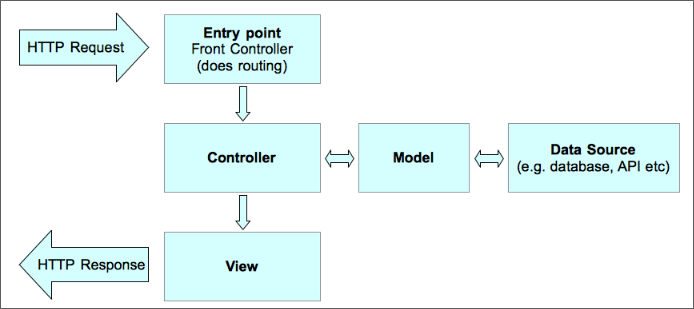
\includegraphics[scale=0.4]{2023_03_09_03_18_14.png}
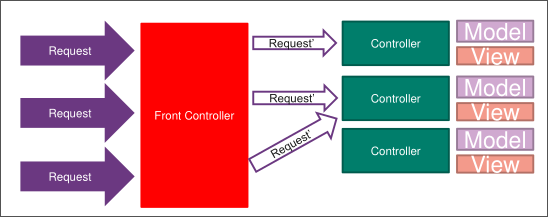
\includegraphics[scale=0.4]{2023_03_09_03_19_43.png}

\subsection{ExpressJS}
\begin{itemize}
\item \textcolor{black}{Most used framework}
\item \textcolor{black}{Javascript}
\item \textcolor{black}{rather old}
\item Integrated Middleware
\end{itemize} 
Base Usage: 
\begin{lstlisting}
import http from 'http';
import express from 'express';

const app = express();
http.createServer(app).listen(3000);

// OR 

import express from 'express';
const app = express();

app.listen(3000, function () {
  console.log('Example app listening on port 3000!');
});
\end{lstlisting}

\subsection{Middleware}
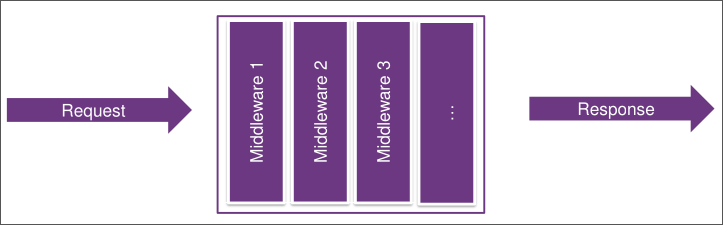
\includegraphics[scale=0.4]{2023_03_09_03_24_51.png}\newline
\textcolor{purple}{Modular components, that will handle individual tasks -> one for authentication, one for authorization.}\newline
\begin{itemize}
\item \textcolor{purple}{Authorization: What am I allowed to do?}
\item \textcolor{purple}{Authentication: Who am I?}
\end{itemize} 

\subsubsection{Usage of Middlewares in ExpressJS}
\textcolor{teal}{In order to register a middleware in expressJS, use the app.use(middleware) function.}
\begin{lstlisting}
import express from 'express';
import bodyParser from 'body-parser';

app.use(express.static(__dirname + '/public'));
app.use(bodyParser.urlencoded({ extended: false }));
app.use(router);

const app = express();
const router = express.Router();
\end{lstlisting}

\subsubsection{Middleware archive "Connect"}
\begin{itemize}
\item \textcolor{purple}{body-parser}
\item \textcolor{purple}{cookie-parser}
\item \textcolor{purple}{cookie-session}
\item \textcolor{purple}{errorhandler}
\item \textcolor{purple}{method-override}
\item \textcolor{purple}{serve-static}
\end{itemize} 

\subsubsection{ExpressJS defaults}
\minipg{
Middlewares:
\begin{itemize}
\item \textcolor{purple}{Router}
\item \textcolor{purple}{Static}
\end{itemize} 
}{
  \textcolor{purple}{Server-Side-Rendering}
}[0.25,0.25]\newline
\minipg{
Request extensions:
\begin{itemize}
\item \textcolor{purple}{params}
\item \textcolor{purple}{is()} -> checks if content-type is correct
\item \textcolor{purple}{get()} -> check header
\end{itemize} 
}{
Response extensions:
\begin{itemize}
\item \textcolor{purple}{sendFile}
\item \textcolor{purple}{format}
\item \textcolor{purple}{json/jsonop}
\end{itemize} 
}[0.25,0.25]

\subsubsection{Routing}
Routers handle requests with endings. This enables you to easily create single page application swith REST.\newline
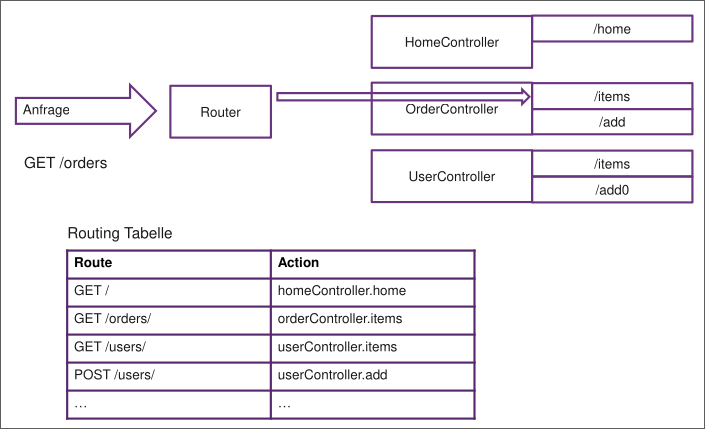
\includegraphics[scale=0.4]{2023_03_09_03_29_44.png}\newline
Setup:
\begin{lstlisting}
import express from 'express';
const router = express.Router();
\end{lstlisting}
Example for \emph{all methods}:
\begin{lstlisting}
router.all('/', function(req, res){
res.send('hello world');
}); // will be called without checking the method
\end{lstlisting}
Example with a specific method
\begin{lstlisting}
router.get('/', function(req, res){
res.send('hello world');
}); // will only be called if it is a get method
\end{lstlisting}
Example with multiple defined methods
\begin{lstlisting}
app.route('/book')
.get(function(req, res) {res.send('Get a random book');})
.post(function(req, res) {res.send('Add a book');})
// used to map multiple methods to one route
\end{lstlisting}

\subsubsection{Route Specifics}
\textcolor{purple}{Router uses pattern matching, this means that you can check for things such as:}
\begin{itemize}
\item \textcolor{black}{/ab*de} -> c or something else implied
\item \textcolor{black}{/*} map to anything
\end{itemize} 
\textcolor{purple}{You can use variables to store requests from users:}
\begin{lstlisting}
router.get('/something/:id', function(req, res) ... // this set the variable id as req.params.id
// note that the req is passed to the function in question, meaning you can handle that variable in that function!
\end{lstlisting}

\subsubsection{Satic-Middleware}
In order to always deliver something like a png, you can use static.
\begin{lstlisting}
app.use(express.static(__dirname + '/public'))
\end{lstlisting}

\subsubsection{Custom Middleware}
In order to create a middleware, you need to use 3 functions/parameters.\newline
The next() has to be called, in order to end the request, otherwise the page will load indefinitely!\newline
Reponse and Request are represented as the res and req in the function.
\begin{lstlisting}
function myDummyLogger( options ) {
  options = options ? options : {};
  return function myInnerDummyLogger(req, res, next) {
    console.log(req.method +":"+ req.url);
    next();
  }
}
\end{lstlisting}

\subsubsection{Error Middleware}
\textcolor{purple}{This should always be registered as the last middleware -> makes sure it catches all errors.\newline
You can however define multiple error middlewares, the last one just needs to end the request.}\newline
\textcolor{teal}{Will be called if an "error-object" is passed to the next() function inside another middleware.}
\begin{lstlisting}
app.use(function(err, req, res, next) {
  console.error(err.stack);
  res.status(500).send('Something broke!');
});
\end{lstlisting}

\textcolor{red}{Note for forms, you can only use the GET and POST methods in forms, this means that something like delete won't work!\newline
\emph{It will be converted to GET requests!}}\newline
As a solution, \emph{use the POST method as a workaround.}

\subsection{Databases and Frameworks}
\textcolor{purple}{You can use any kind of databases like SQL -> Postgres, NoSQL, JSON, in memory databases etc.}

\subsubsection{Example with nedb (NoSQL)}
\begin{lstlisting}
import Datastore from '@seald-io/nedb';
const db = new Datastore({filename: './data/order.db', autoload: true});

// insert 
db.insert(order, function(err, newDoc){
  if(callback){
    callback(err, newDoc);
  }
});

// find or findOne
db.findOne({ _id: id }, function (err, doc) {
  callback( err, doc);
});

// update 
db.update({_id: id}, {$set: {"state": "DELETED"}}, {}, function (err, doc) {
  publicGet(id,callback);
});
\end{lstlisting}

\subsubsection{Templating engine with DatabaseTemplating engine with Databasess}
The question is, how do we generate html when we want to do it dynamically? \newline
Meaning how do we interact with html and database? Templates!\newline
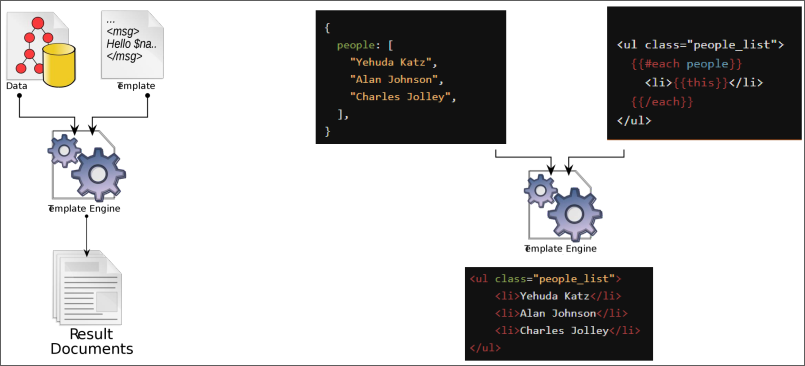
\includegraphics[scale=0.4]{2023_03_09_04_28_05.png}
\begin{itemize}
\item \textcolor{black}{definition of look -> handlebar framework language}
\item \textcolor{black}{definition of tables -> json}
\item \textcolor{black}{caching}
\item \textcolor{black}{Partials}
\item converts html and json to the result document.
\end{itemize} 

\subsubsection{Handlebars template engine}
Exmple for handlebars: \newline
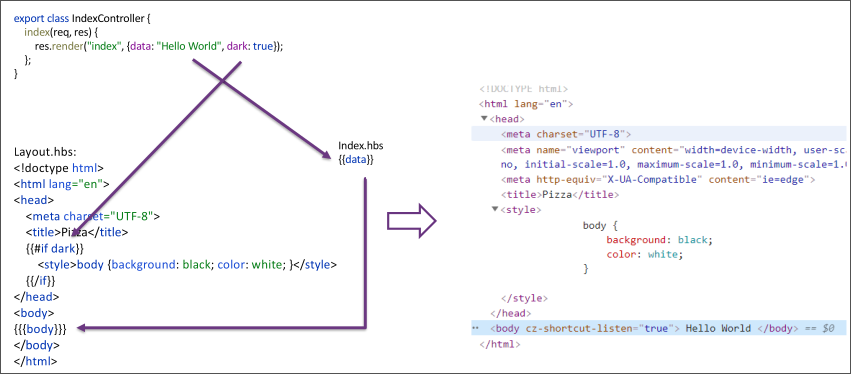
\includegraphics[scale=0.4]{2023_03_09_04_37_20.png}\newline
\begin{lstlisting}
// 1. import express-handlebars
import exphbs from 'express-handlebars';

const app = express();

// 2. configure
const hbs = exphbs.create({
  extname: '.hbs',
  defaultLayout: "default",
  helpers: {
    ...helpers
  }
});

// 3. set engine and global values
app.engine('hbs', hbs.engine);
app.set('view engine', 'hbs');

// 4. path to views
app.set('views', path.resolve('views'));

// usage afterwards
// app.render(view, [locals], callback)
createPizza = async (req, res) => {
  res.render("succeeded", await orderStore.add(req.body.name, "unkown"));
};
\end{lstlisting}

\begin{lstlisting}
<p>Order-Informationen</p>
{{#if pizzaName}}
  <p>Bestellte Pizza: {{pizzaName}}</p>
  {{#if_eq state "OK"}}
    <form action='/orders/{{_id}}' method='post'><input type='hidden' name='_method' value='delete'><input
      type='submit' value='Delete order'></form>
  {{/if_eq}}
{{/if}}

// render 
async showOrder(req, res) {
  res.render("showorder", await orderStore.get(req.params.id));
};
\end{lstlisting}
\textcolor{purple}{You can also send data to the template from within javascript}\newline
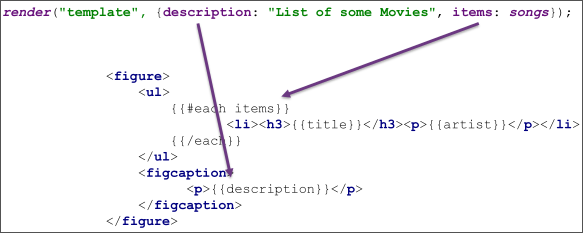
\includegraphics[scale=0.4]{2023_03_09_04_32_07.png}\newline
\textcolor{purple}{In loops, the current object is the current context:}\newline
\begin{lstlisting}
<ul>
  {{#each items}}
  <li>
    <h3>{{title}}</h3>
    <p>{{this.artist}}</p>
  </li>
  {{/each}}
</ul>
// you can access the root with {{@root}}
\end{lstlisting}

\textcolor{purple}{Handlebars only defines a few helpers (functions), but you can define some yourself!}
\begin{lstlisting}
//Usage: {{? hasError 'error' 'ok'}}
Handlebars.registerHelper('?', function(exp, value1, value2, options) {
  if(exp) {
    return value1;
  }
    return value2;
  });
{{? hasError 'FEHLER' 'OK' }}
\end{lstlisting}

\subsection{Security with ExpressJS}
\subsubsection{Authentication with Cookies}
Cookies represent a small piece of data. This can be a state in which the website was in before the client left the last time.\newline
Data is represented as a key=value pair.\newline
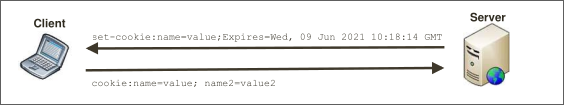
\includegraphics[scale=0.4]{2023_03_16_03_17_28.png}\newline
Usage: \newline
\textcolor{purple}{npm install cookie-parser -save \newline
app.use(require("cookie-parser"){} );}

\subsubsection{Session with Cookies}
Usage:\newline
\textcolor{purple}{npm install session-parser -save\newline
app.use(session((secret: ,'1234567', resave: false, saveUninitialized: true)));}\newline
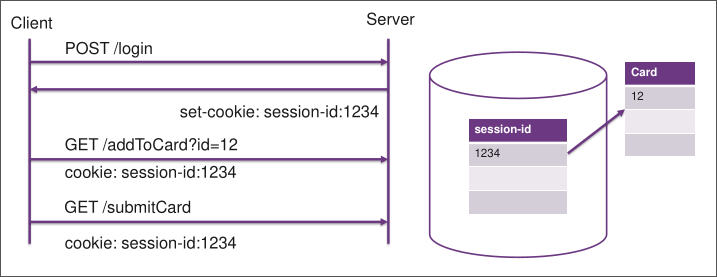
\includegraphics[scale=0.4]{2023_03_16_03_20_23.png}

\subsubsection{Storing cookies}
\textcolor{purple}{Cookies (more likely its data) are often stored in json, this can be done as follows}\newline
\begin{lstlisting}
// valid but dangerous
JSON.stringify([1,2,4,5]);
// better:
json = JSON.stringify({elements : [1,2,4,5]});

// get the elements again with 
elements = JSON.parse(json); 
\end{lstlisting}

\subsection{REST with Cookies}
\textcolor{purple}{The problem is that with REST we want a stateless connection, this means that we need to change the way data is transferred, by changing the format.}\newline
\begin{lstlisting}
res.format({
  'text/html': function () {
    res.redirect("/");
  },
  'application/json': function () {
    res.send(true);
  },
});
\end{lstlisting}
\textcolor{teal}{The problem is that now, because of the stateless connection, we need to send all data each time.\newline
For example you would need to send something like a \emph{token} to login. -> see discord and why you can create bridges.}\newline
Token requirements:
\begin{itemize}
\item \textcolor{purple}{creation date }
\item \textcolor{purple}{expiry date }
\item \textcolor{purple}{signature}
\item \textcolor{purple}{Other data that might help protect user and server}
\end{itemize} 
\minipg{
\begin{itemize}
\item \textcolor{green}{Connection can be sent to any server!}
\end{itemize} 
}{
  \begin{itemize}
  \item \textcolor{red}{What happens if the token gets stolen?}
  \item \textcolor{red}{What happens when a device gets stolen? \newline
    How would we invalidate the token on it?}
  \end{itemize} 
}[0.25,0.25]
\textcolor{teal}{Tokens can be used either as a pseudo key, which can be used to connect to services, or as a temporary login -> remember that you are logged in for a while. RIGHT MOODLE??}\newline
Libraries:
\begin{itemize}
\item \textcolor{black}{oauth}
\item \textcolor{black}{express-jwt}
\item \textcolor{black}{node-jsonwebtoken}
\end{itemize} 

\subsubsection{JWT Token}
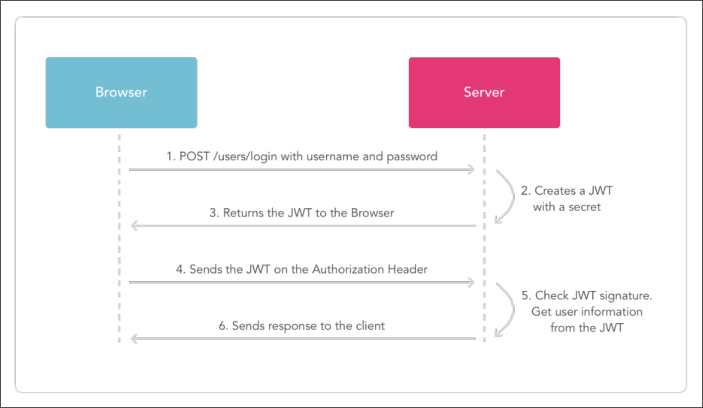
\includegraphics[scale=0.4]{2023_03_16_03_56_53.png}
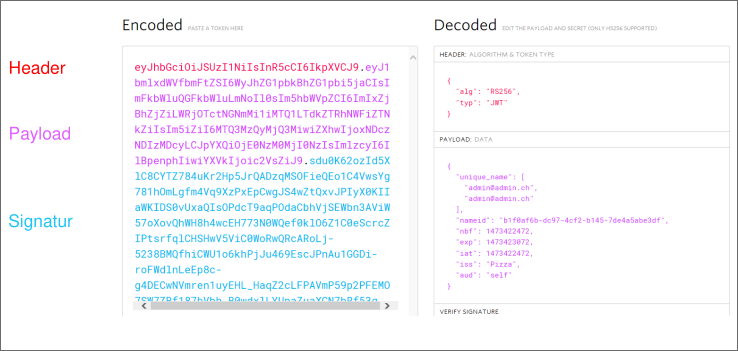
\includegraphics[scale=0.4]{2023_03_16_03_56_22.png}

\subsection{AJAX}
\textcolor{purple}{When using ajax on webpages, make sure to change the state of the application so that a redo or undo button doesn't end redirecting you back to google. \newline
As an alternative use frameworks like react which do this automatically.}
\begin{lstlisting}
history.pushState({}, "Demo", "bar.html");
\end{lstlisting}

\subsection{Fetch}
\begin{lstlisting}
fetch(url, {
  method: method,
  headers: {
    'Content-Type': 'application/json'
  },
  body: JSON.stringify(data)
}).then(x => {
  return x.json();
});
\end{lstlisting}
Possible other data: 
\begin{itemize}
\item \textcolor{purple}{arrayBuffer()}
\item \textcolor{purple}{blob()}
\item \textcolor{purple}{formData()}
\item \textcolor{purple}{text()}
\end{itemize} 

\subsubsection{Cookies with Fetch}
Cookies aren't sent automatically, this means you have to send them alongside!
\begin{lstlisting}
fetch('https://example.com', {
  credentials: 'include'
})
\end{lstlisting}

\subsubsection{Fetch helper classes for requests}
\begin{lstlisting}
const myHeaders = new Headers();
myHeaders.append('Content-Type', 'text/plain');
const myInit = {
  method: 'GET',
  headers: myHeaders,
  cache: 'default'
};
const myRequest = new Request('/example', myInit);
fetch(myRequest) /*…*/
\end{lstlisting}

\subsection{CORS}
\textcolor{purple}{AJAX security feature. It basically says that a client may only request ajax promises from the one main server.}\newline
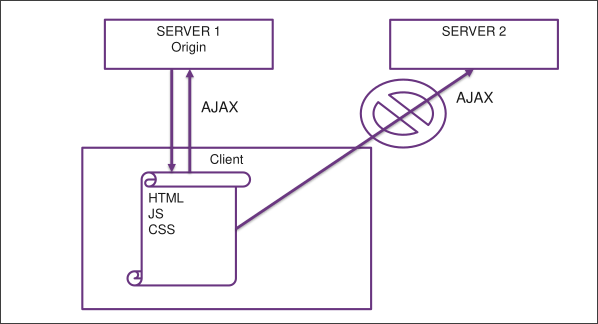
\includegraphics[scale=0.4]{2023_03_16_04_32_40.png}\newline
\textcolor{purple}{You can define yourself, who exactly is allowed use what type of functions.}
\begin{lstlisting}
const allowCrossDomain = function(req, res, next) {
  res.header('Access-Control-Allow-Origin', '*');
  res.header('Access-Control-Allow-Methods', 'GET,PUT,POST,DELETE');
  res.header('Access-Control-Allow-Headers', 'Content-Type');
  next();
};
app.use(allowCrossDomain);
\end{lstlisting}

\section{Typescript}

\subsection{Motivation}
\begin{itemize}
\item \textcolor{black}{types...}
\item \textcolor{black}{actual help in IDEs -> does the function or variable actually exist?}
\item \textcolor{black}{Warns when types do not match, as said actual types!}
\item \textcolor{black}{object Object}
\end{itemize} 

\subsection{Configuration}
\textcolor{teal}{Each typescript project needs a config file that defines how tsc will compile the files back to js.}
\begin{lstlisting}
// tsconfig.json
{
  "compilerOptions": {
    "target": "ES6",
    "module": "ES6",
    "moduleResolution": "Node",
    "allowJs": true,
    "checkJs": true,
    "strict": true,
    "esModuleInterop": true
  },
  "exclude": [
    "node_modules"
  ]
}
\end{lstlisting}

\subsubsection{Import of JS module types}
\textcolor{teal}{One problem that we have is that the js modules have their own classes etc, these are obviously not included in ts and therefore need a special module import.\newline
For example if you use express, then you need to install express types as well: \emph{npm i --save-dev @types/express}}

\subsubsection{Prettier}
Theoretically it is necessary to use these plugins, but nvim fucking rocks so no need. 
\begin{lstlisting}
{
  "parser": "@TypeScript-eslint/parser",
  "plugins": [
    "@TypeScript-eslint"
  ],
  "extends": [
    "plugin:@TypeScript-eslint/recommended"
  ]
}
\end{lstlisting}

\subsection{Types}

\subsubsection{Primitives}
\begin{itemize}
\item \textcolor{purple}{boolean}
\item \textcolor{purple}{number: yes number... -> i32,i64,u32,u64..}
\item \textcolor{purple}{string}
\item \textcolor{purple}{null: WHY}
\item \textcolor{purple}{undefined}
\item \textcolor{purple}{void: special type}
\item \textcolor{purple}{never: special type}
\item \textcolor{purple}{any: like js but only in non strict mode!}
\end{itemize} 

\subsubsection{Strict Mode}
\textcolor{purple}{"strict"=true in the config file makes sure that the any keyword can't be used for variables!}\newline
Strict also has the following results:
\begin{itemize}
  \item NoImplicitThis: this needs to be used explicitly
  \item strictBindCallApply
  \item strictFunctionTypes
  \item strictPropertyInitialization: properties of classes need to be initialized -> like rust.
\item \textcolor{black}{NoImplicitAny: you need to explicitly write any}
\item \textcolor{black}{alwaysStrict: set in the first line of a file}
\item \textcolor{black}{strictNullChecks: null and undefined are no longer base types -> can't be assigned!}
\item \textcolor{black}{item 4}
\end{itemize} 

\subsubsection{Collection Types}
\begin{lstlisting}
let myInferredNumArray = [1, 2, 3];
let myNumArray: number[] = [1, 2, 3];
// let myNumArray: Array<number> = [1, 2, 3]; // same as above but explicitly
let myTupel = [1, "abcd"]
// problem with this -> myTupel[1] = 2; would work since it can't see type, use the one below to avoid this
let myTupel: [number, string] = [1, "abcd"]   // same as above but explicitly
\end{lstlisting}

\subsubsection{Union Types}
\textcolor{teal}{Similat to C, unions are a space that can be interpreted as multiple types.}
\begin{lstlisting}
let something = string | number; // can be either a number or a string.
something = "pinpang"; // ok
something = 50; // ok
\end{lstlisting}

\subsubsection{Type Narrowing}
Due to the fact that a variable might have multiple types, you need to make sure that the type has the correct type for a certain operation at the time:
\begin{lstlisting}
// Type Narrowing - due to assignment
let myVar3: string | number;

// not allowed
console.log(myVar3 / 3)
// allowed
myVar3 = 9;
console.log(myVar3 / 3)

// Type Narrowing - due to condition interpretation
function typeNarrowingFn (myParam: string | number) {

  // not allowed
  console.log(myParam / 3)
  // allowed
  if (typeof myParam === "number") {
    console.log(myParam / 3)
  }
}
\end{lstlisting}

\subsubsection{Function declarations and definitions}
\begin{lstlisting}
function add(s1: string, s2: string): string; // function with 2 parameters and return type of string
function add(n1: number, n2: number): number; // function with 2 parameters and return type of nubmer
function add(n1, n2) {
  return n1 + n2;
} // inferred return type

// this function has an optional parameter -> this is annotated with the ? symbol
function combineFunction(sn: number | string = "", ns?: number): string {
  return String(sn) + String(ns || ""); // the double pipe represents the OR as it needs a fallback
  // aka if ns is undefined use the other one
}
// allowed
let myNum: number = add(1, 2);
combineFunction(1);
\end{lstlisting}
\textcolor{teal}{Note, when using the optional parameter, you always need a fallback for this parameter should it not be passed. \newline
Alternatively, and probably \emph{preferably}, use optional parameters with \emph{a default fallback value!}}
\begin{lstlisting}
  // here the function takes 2 parameters with the second one being 10 if it is not provided!
  function something(a: number, b = 10 ): number {
    return a + b; 
  }
\end{lstlisting}
Obviously, you can also use functions as parameters:
\begin{lstlisting}
function numberApplicator(numArray: number[],
                          numFun: (prevRes: number, current: number) => number): number {
  return numArray.reduce(numFun);
}
\end{lstlisting}

\subsubsection{Classes}
\textcolor{purple}{private variables can be defined either with the private keyword, or with a \#.}\newline
You can of course declare and instantly assign variables in typescript, apparently that was not a thing in js for a while...
\begin{lstlisting}
class Counter {
  #doors: number; // ES2022 private field
  private wood: string = "oak"; // TS private fields
  something?: number; // optional field
  public static readonly WOOD_FACTORS = {'oak': 80, 'pine': 20};

  // readonly -> const
  // # -> private
  // ? -> optional
  // private -> private
  
  constructor({doors = 2}: {doors?: number} = {}) {
    this.#doors = doors;
  }
  set doors(newDoorCount: number) { // ES6 setter
    if (newDoorCount >= Counter.MIN_DOOR_COUNT && newDoorCount <= Counter.MAX_DOOR_COUNT) {
    this.#doors = newDoorCount;
    } else {
      throw 'Counter can only have';
    }
  }
  get doors() {
    return this._doors;
  }
}

// You can also define new properties right in the constructor. 
// !!initialization is made automatically!!
class SportsCar {
  constructor(
    public make: string,
    public color: SportsCarColor,
    public gears: number,
  ) {}
}
\end{lstlisting}

\subsubsection{Interfaces}
\begin{lstlisting}
interface IPoint {
  readonly y: number;
} 

interface IPoint {
  readonly x: number;
} // adds value to previous interface

interface ILikableItem {
  likes?: number;
} // optional entry

class DescribableItem {
  constructor(
    public description: string
  ){}
} 
class PointOfInterest extends DescribableItem implements IPoint, ILikableItem {
  constructor(public x: number, public y: number, description: string, public likes?:number) {
    super(description);
  }
}
\end{lstlisting}

\subsubsection{Types}
\textcolor{teal}{You can create types that can later be used in variables:}
\begin{lstlisting}
type Shape =
{ kind: "circle"; radius: number }
| { kind: "rectangle"; w: number; h: number }
| { kind: "square"; size: number };

let something: Shape = {kind: "circle", radius: 10}
\end{lstlisting}
\textcolor{red}{Keyof}: This takes the underlying types of a type and copies them into another
\begin{lstlisting}
type Point = { x: number; y: number };
type P = keyof Point;
// P has the same types -> Point

type Mapish = { [k: string]: boolean };
type M = keyof Mapish;   
// type M = string | number

// You can also create something similar to a grammar:
type Shipper = 'UPS' | 'FEDEX' | 'DHL';
type TrackingType = 'Overnight' | 'Priority' | 'Economy';
\end{lstlisting}

\subsubsection{Casting}
Just like in rust -> 42 as i64
\begin{lstlisting}
const myCanvas = document.getElementById("main_canvas") as HTMLCanvasElement;
\end{lstlisting}

\subsubsection{Explicit Null}
Don't use this..
\begin{lstlisting}
function countLines(text?: Array<string | null>): number {
  let count = 0;
  for (const line of text || []) {
    if (line && line.length !== 0) {
      count += 1;
    }
  }
  return count;
}
const a = countLines(["one", "two", "three", ""]);
const b = countLines(["one", null, "three"]);
\end{lstlisting}

\subsubsection{Generics}
\begin{lstlisting}
function identity<Type>(arg: Type): Type {
  return arg;
}
// or in case of arrays
function loggingIdentity<Type>(arg: Type[]): Type[] {
  console.log(arg.length);
  return arg;
}
// or a class
class GenericNumber<NumType> {
  zeroValue: NumType;
  add: (x: NumType, y: NumType) => NumType;
}
\end{lstlisting}

% \lstset{
%     language=TypeScript,
%     style=code,
% }

\lstset{
    language=CSS,
    style=code,
}

\lstset{
    language=HTML,
    style=code,
}

\end{document}
